\chapter{Literature Review}
\label{chap2}

\section{Introduction}

In this chapter, previous work and research that has been performed in the fields relevant to this project is mentioned and discussed. These fields include the quadcopter platform, computer vision and machine learning techniques. 

\section{Quadcopters}

A quadcopter is an autonomous aerial vehicle (UAV) in a four-arm frame configuration. This configuration comes in an X or plus (+) shape, with the control equipment and sensors typically located at the centre of the frame. See Figure~\ref{fig:chap2-quad} for a picture of the SunKopter in a typical quadcopter X configuration. They can also come equipped with either four or eight motors and props, though the four-rotor variant is very common.

\begin{figure}
  \centering
  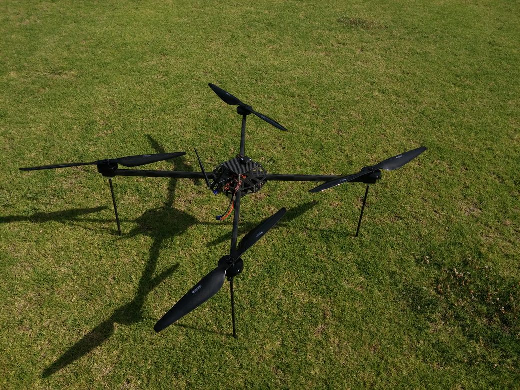
\includegraphics[clip, trim = 0 0 30 20, width=0.5\textwidth]{figures/chapter2/quadcopter}
  \caption[A picture of the SunKopter, as used by STERG.]{A picture of the SunKopter, as used by the Solar and Thermal Energy Research Group.}
\label{fig:chap2-quad}
\end{figure}

Quadcopters move in three-dimensional space and have six degrees of freedom: three in the translation space ($x, y, z$) and three in rotation space ($\theta, \phi, \psi$), where the rotations are defined by an Eulerian aeroplane angle scheme, i.e.\ roll, pitch and yaw angles. The rotors on each axis of the frame rotate in the same direction, with each axis' rotating in opposite directions relative to one another. See Figure~\ref{fig:chap2-quad-rotation} for a diagram demonstrating this. 

\begin{figure}
  \centering
  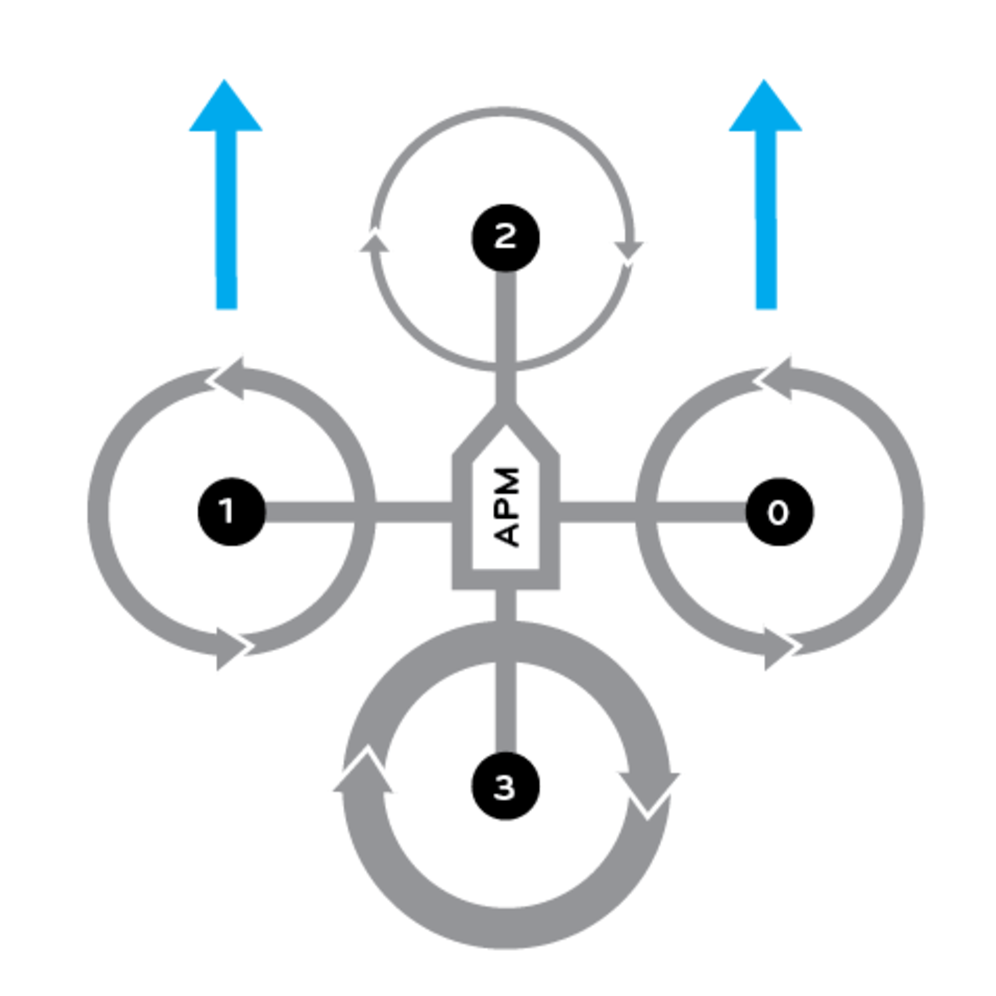
\includegraphics[width=0.5\textwidth]{figures/chapter2/quad_axis.pdf}
  \caption[Diagram presenting the opposing axis rotations directions.]{Diagram presenting the opposing axis rotation directions. The thickness of the arrows represent the power output of the motor.~\cite{quad-rotation-pic}}
\label{fig:chap2-quad-rotation}
\end{figure}

Movement in each of the six directions is achieved as follows:

\begin{enumerate}
  \item Forward/backward or left/right movement: Keep one axis' motor speed constant, while raising and lowering the motor speed of the motors on the other axis (demonstrated in Figure~\ref{fig:chap2-quad-rotation}).
  \item Higher/lower: Increase or decrease all of the motor speeds to increase or decrease the altitude.
  \item Roll/pitch: Same process as for linear movement.
  \item Yaw: Collectively increase or decrease the motor speed of one axis relative to the other. 
\end{enumerate}

As described in Chapter REF CHAP1, the goal of this project is to determine the pose estimation error, i.e.\ the difference between a quadcopter's true pose and its estimated pose. To be able to do this, it is important that the dynamics and control strategies of a typical quadcopter is well defined and understood. This section sets out to discuss the dynamic modelling of a quadcopter, as well as the different control strategies that have been developed and implemented in the past. 

\subsection{Plant Modelling}

When designing a control system, arguably the most crucial part of the design process is to derive an accurate mathematical model of the plant that is to be controlled. The plant in this case is a UAV in a quadcopter configuration. 

As part of their X-4 Flyer project,~\cite{hamel2002dynamic} set out to derive a simple model for their plant using only rigid body dynamics and abstract force and torque actuators. As stated by~\cite{Pounds2010c}, this model, like many others that were derived at the time, represents the quadcopter as a rigid body mass with inertia and autogyroscopics, affected only by gravity and actuator torques.~\citeauthor{Pounds2010c} further argues that these simple quadcopter models do not accurately represent the complex helicopter-like behaviour exhibited by real quadcopters at high rotor speeds. These high-speed rotor effects include the blade flapping effect, which affect the quadcopter frame's oscillatory modes, rotor flapping from varying quadcopter yaw angles, and variable airflow velocities over the rotor blades from varying roll and pitch angles.

In an attempt to create a more accurate quadcopter model that will allow a quadcopter to be more accurately controlled at high rotor speeds,~\citeauthor{Pounds2010c} set out to derive a model incorporating the rigid body dynamics, as well as the aerodynamic effects mentioned earlier. Their model is based in part on the diagram given in Figure~\ref{fig:chap2-quad-model}.

\begin{figure}
  \centering
  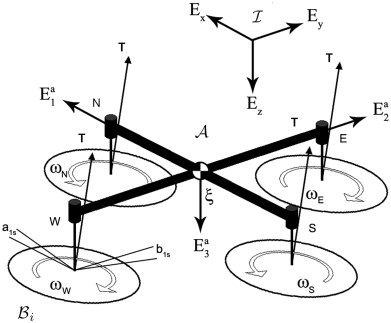
\includegraphics[width=0.5\textwidth]{figures/chapter2/pounds_quad-model.jpg}
  \caption[A diagram of the quadcopter model, including the blade flapping dynamics.]{A diagram of the quadcopter model, including the blade flapping dynamics as presented by~\cite{Pounds2010c}.}
\label{fig:chap2-quad-model}
\end{figure}

Their resulting model was used to develop a simple hovering Proportional Integral Differential (PID) attitude and altitude controller for the purpose of model verification. The results show that the drone stabilised itself in indoor flight with $\pm1$\textdegree\ of precision and $\pm5$\textdegree\ of precision during outdoor flight. The lower precision during outdoor flights is due to the added wind disturbances, etc. Thus, the model, as it stands, is sufficiently accurate to safely control a drone for hovering. However, they did not compare their model, which includes aerodynamic effects, against the model of~\citeauthor{hamel2002dynamic}, which is based solely on rigid body dynamics. 

\subsection{Control Strategies}

\subsubsection{Introduction}

After an accurate model, the next most important part of a good control system is the controller itself. Many controllers have been implemented and tested on quadcopters over the years. Different control strategies have also been investigated. Some of the most prevalent control strategies and controllers are discussed here.

\subsubsection{Indoor vs. Outdoor Control}

There are different types of quadcopters, each of them equipped with different sensors and equipment. However, two types of quadcopter with distinct sensor and control approaches are relevant here. They are the indoor and outdoor quadcopters. Each of them work in different ways and implement very different control schemes. 

Indoor drones may or may not come equipped with an on-board inertial measurement unit (IMU), which includes an accelerometer and gyroscope, for stability control. However, they commonly solely rely on an external motion detection system which tracks the drone, providing position and rotation (also known as pose) feedback to the controller, thereby closing the feedback control loop. These drones are exceptionally accurate thanks to the high accuracy of their external motion sensing equipment, and are capable of performing remarkable acrobatic feats. However, their use is restricted to carefully regulated and controlled indoor environments.

Outdoor drones, without the luxury of having very accurate external sensors available, have to rely on their on-board sensors to provide the controller with pose feedback. The on-board sensors these drones come equipped with may vary between quadcopter platforms, however they almost certainly come equipped with an IMU to provide pose data. However, since the IMU readings for position data drifts with time due to integration errors, a global positioning system (GPS) sensor is added to provide a base-line reading of a quadcopter's position. Other sensors that may be included are magnetometers, barometers, visual feedback sensors and sonar sensors. To combine the readings of the different sensors, a filtering technique, such as the Extended Kalmann Filter, is used. The pose error of the combination of the different readings are, in theory, less than the most accurate sensor in the suite, but this has not yet been proven and an exact error margin is yet to be determined. 

\subsubsection{Hovering Control}

The stable hovering of a quadcopter has been the focus of many projects and research papers in the past 15 years. As a result, many different control methods and schemes have been investigated, implemented and compared. Hovering control refers to a quadcopters ability to hover and remain stable at a set point in three-dimensional space.

\cite{bouabdallah2004pid}, as part of their `OS4' project, compared the modern linear quadratic regulator (LQR) and classic PID controller, with respect to the control performance (disturbance rejection, reference tracking, etc.) of a quadcopter.

They found that the PID controller produced better results than the LQR in terms of reference tracking and dynamic performance. This was a surprising result, since LQR controllers normally excel at controlling unstable, underactuated plants such as a quadcopter platform. They suspect that the reason for this result may be because the PID controller is better at handling plant uncertainties, since they neglected the effects of actuator dynamics such as blade and rotor flapping, in their drone model. They do expect that an LQR controller will produce superior results if a more accurate model is used by taking these effects into account. 

Some researchers have also investigated controlling a drone using an H-infinity (H$_{\inf}$) control structure and a model predictive controller (MPC). Most notably,~\cite{raffo2010integral} have done extensive research on this topic. MPC's are computationally efficient and modern controllers that drive a plant's state to a reference state within predefined constraints (eg.\ motor saturation, model dynamics, etc.), while a properly designed non-linear H$_{\inf}$ controller is very good at rejecting disturbances (eg.\ wind gusts, motor vibrations, etc.) and are robust to model uncertainties. They opted to combine the two controllers in an intelligent manner in order to extract the most efficient performance from their drone. 

In their simulations they found that the resulting controller performed admirably, presenting good reference tracking, proving to be robust with uncertain mass and inertia terms and deals well with disturbances on all six degrees of freedom at different points in time. However, they are yet to implement and test their controller configuration on a real drone. Although the algorithms and methods they used are computationally efficient, it may still prove to be too computationally intensive for the limited computing power on-board a drone. Given the fast growth of processing power, however, this controller configuration may become a more viable option in the near future. 

Controllers for enabling a drone to hover have already been successfully designed and implemented, and it is therefore possible to stabilise and accurately control a drone during hovering operations. 

\section{Computer Vision}

\subsection{Introduction}

Computer vision is a diverse field which primarily focuses on devising methods for acquiring, processing, analysing and understanding images captured of the real world. There are various sub-fields of research, but a common theme across all the fields is to mimic the human ability to perceive and understand an image, and illicit an appropriate reaction to different visual inputs. 

The fields of interest for this thesis, are the object detection, tracking and pose estimation fields. This section aims to discuss the work that has been performed in these fields. 

\subsection{Camera Matrix}

A digital image is a collection of two-dimensional colour intensity vectors representing a collection of three-dimensional space vectors. These collections of vectors are related by a matrix $C$, known as the camera matrix. The camera matrix contains the intrinsic parameters of the camera that recorded the image, i.e.\ the focal lengths and principle point of the image, as well as the extrinsic, or pose, parameters of the camera, i.e.\ the translation and rotation information. The camera matrix $C$ given is given by Equation~\ref{eq:chap2-cam-matrix}, as derived by~\cite{heikkila1997four}

\begin{equation}
  \label{eq:chap2-cam-matrix}
  C = 
  NP
\end{equation}

where $N$ is given by the matrix in Equation~\ref{eq:chap2-cam-intrinsic}.

\begin{equation}
  \label{eq:chap2-cam-intrinsic}
  N = 
  \begin{bmatrix}
    f_x & 0   & u_0 \\
    0   & f_y & v_0 \\
    0   & 0   & 1   \\
  \end{bmatrix}
\end{equation}

Here, $f_x$ and $f_y$ describe the focal lengths of the camera and $u_0$ and $v_0$ are the camera's principal points. The pose matrix $P$ is given by the matrix in Equation~\ref{eq:chap2-cam-extrinsic}.

\begin{equation}
  \label{eq:chap2-cam-extrinsic}
  P = 
  \begin{bmatrix}
    R | T
  \end{bmatrix}
  =
  \begin{bmatrix}
    r_{11} & r_{21} & r_{31} & t_1 \\
    r_{21} & r_{22} & r_{32} & t_2 \\
    r_{31} & r_{23} & r_{33} & t_3 \\
  \end{bmatrix}
\end{equation}

In the matrix $P$, $R$ is a $3\times3$ matrix describing the rotation of the camera, and $T$ is a three-dimensional vector describing the translation of the camera. The pose information is given relative to some reference object or plane in the image. 

The two-dimensional image projection of an object in three-dimensional world space is related through the camera matrix $C$ with the relation given in Equation~\ref{eq:chap2-2d-to-3d}. The camera matrix is commonly determined through some camera calibration procedure. One such a procedure is discussed in Section~\ref{sec:chap2-cam-calibration}.

\begin{equation}
  \label{eq:chap2-2d-to-3d}
  x_c
  = C
  X_w
\end{equation}

where $x_c$ is a homogeneous image vector $[x\;y\;1]$ and $X_w$ is a homogeneous world coordinate vector $[X\;Y\;Z\;1]$. 

\subsection{Camera Calibration}
\label{sec:chap2-cam-calibration}

A properly calibrated camera is a very important part of any computer vision system, since the accuracy of the data extracted from an image strongly depends on the accuracy of the calibration procedure and results. The goal of a camera calibration procedure is to produce the complete camera matrix $C$, as given in Equation~\ref{eq:chap2-cam-matrix}, as well as finding the camera's distortion coefficients introduced by low-quality or fish-eye lenses. There are various camera calibration procedures available, from the two-step calibration described by~\cite{melen1994geometrical} to the classical approach given by~\cite{slama1980manual}, where a non-linear error function is minimised. However, the minimisation problem presented by~\citeauthor{slama1980manual} is computationally inefficient and slow, while~\citeauthor{melen1994geometrical}'s method does not account for image distortion and correction. A popular calibration method is the four-step method, proposed by~\cite{heikkila1997four} as an extension to the two-step method which was the prevalent calibration procedure at the time.

The `calibrateCamera()' function of the OpenCV computer vision library [\cite{bradski2000opencv}], makes use of the four-step method.\footnote{The version used is OpenCV v2.4.8} The fine details of the method is beyond the scope of this research, however a broad overview of the steps and equipment required to calibrate a camera, is provided. 

To perform the calibration and find the camera matrix, OpenCV requires two sets of data: one two-dimensional image data set, $x_c$, as well as a set of corresponding three-dimensional data points, $X_w$. This implies that image data of an object where the dimensions and coordinates of certain features are known, must be recorded. In practice, any well-characterised object can be used for calibration. For example, some calibration methods rely on a three-dimensional cube covered in precisely laid out markers. However, since manufacturing and distributing such precisely constructed objects to a large audience is infeasible, OpenCV opts to use a more convenient flat, regular pattern, such as chessboard or asymmetrical dot pattern. Figure~\ref{fig:chap2-calib-pattern} shows an example of a typical chessboard pattern generated by OpenCV.\@ With these flat patterns, the features used to populate the data sets would be the square corners on a chessboard, i.e.\ where a black block meets another black block, or the dots on an asymmetric dot pattern. The drawback to this approach, however, is that multiple views of the flat calibration pattern is required, whereas a single image of a three-dimensional object would suffice. However, more data points would allow the optimisation procedure built into the algorithm to find a more accurate result.  

\begin{figure}
  \centering
  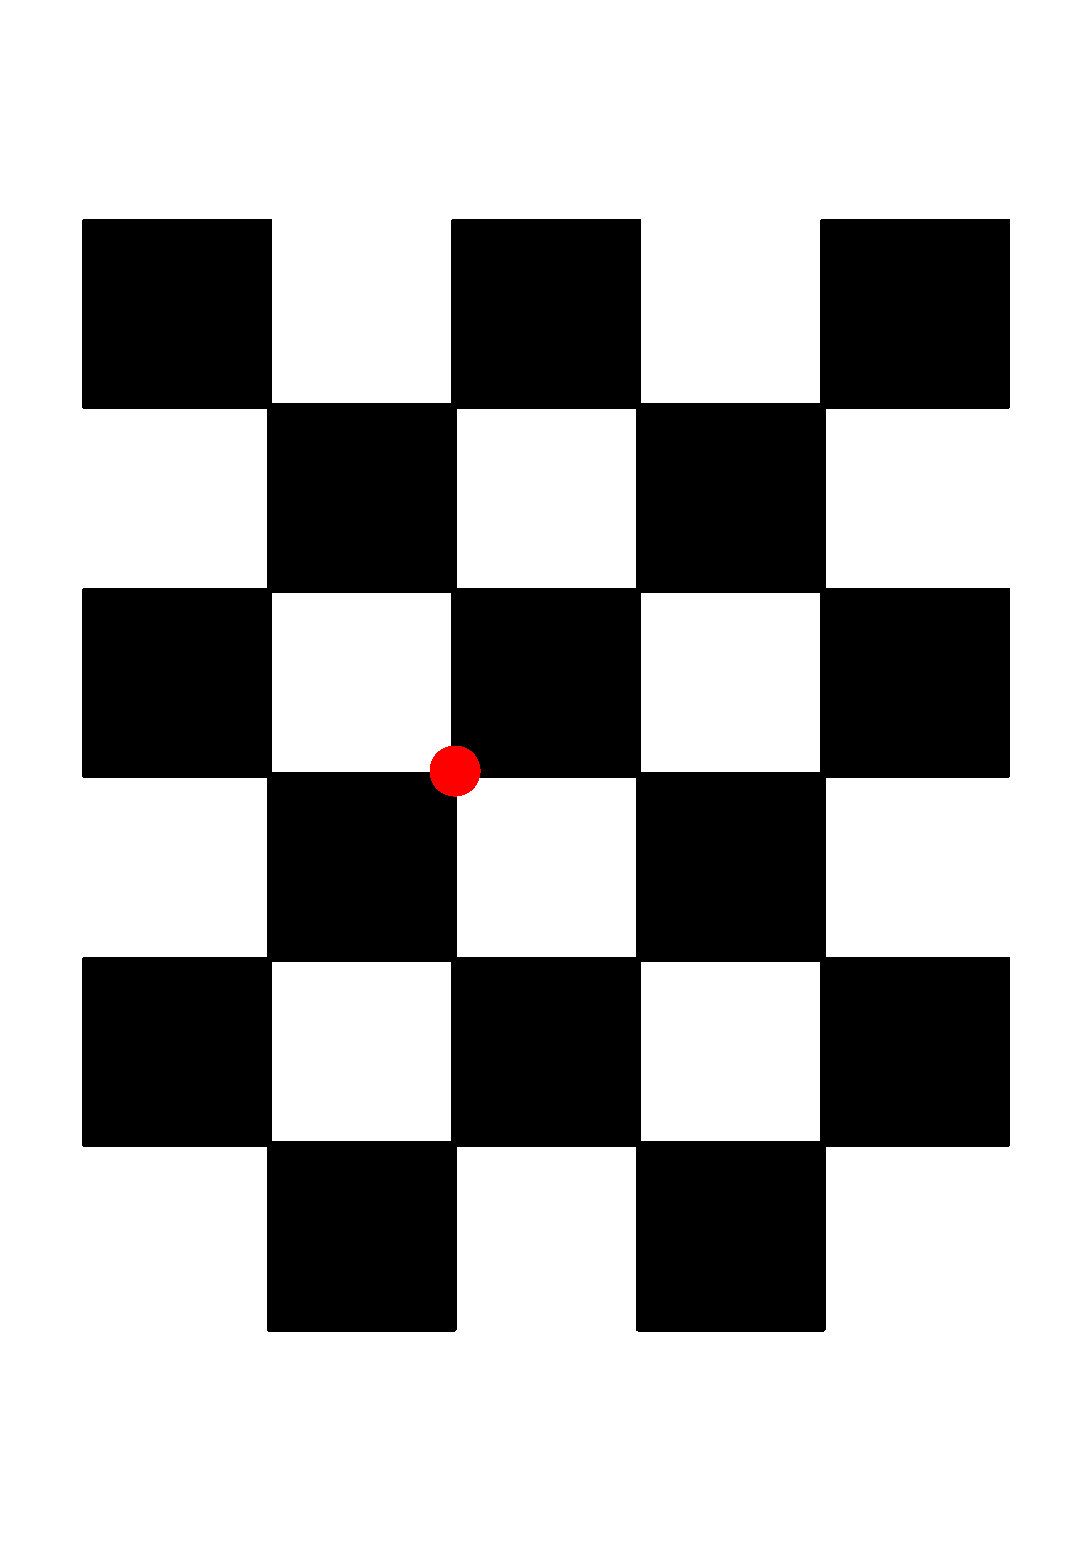
\includegraphics[angle=90, width=0.5\textwidth]{figures/chapter2/chessboard_pattern}
  \caption{An example of a typical chessboard pattern used for calibration.}
\label{fig:chap2-calib-pattern}
\end{figure}

In the case of the chessboard pattern, acquiring the two-dimensional pixel coordinates of the corners is accomplished by using OpenCV's `findChessboardCorners()' and `findCornerSubPix()' functions, which makes use of a Harris corner detection algorithm, first described by~\cite{harris1988combined}. The three-dimensional world coordinates of the features is fed to the calibration function according to an axis-system and measurement unit defined by the programmer. These coordinates can be as simple as a vector containing the feature coordinates in square units, for example the corner from Figure~\ref{fig:chap2-calib-pattern} will then be represented as $(3, 2, 0, 1)$ in homogeneous coordinates (note that $z_w$ will be zero since the board is flat). 

Next, for best calibration results, OpenCV recommends that camera calibration take place within a well-lit room with a white background, using a calibration pattern with a wide white border in clear view of the camera and at different locations and orientations relative to the camera. These recommendations are mainly to increase the contrast between the black features and the white background and make it easier for OpenCV to accurately find each feature's pixel coordinates. Furthermore, the more diverse the location and orientation data is, the more accurate the estimate for the intrinsic camera parameters will be. 

With the of two-dimensional and three-dimensional data sets now known, the calibration function can determine the camera matrix $C$. 

\subsection{Principle n-Points Problem}

The Principle n-Points (PnP) problem, as stated by~\cite{horaud1989analytic}, `is the problem of finding the position and orientation of a camera with respect to a scene object from $n$ correspondence points', where the scene object would normally be a well-characterised calibration object or pattern. It is a well-researched sub-field of computer vision with various solutions to the problem that have been proposed. These solutions include some non-iterative solvers, such as the P3P solution proposed by~\cite{gao2003complete} and the PnP solvers by~\cite{lepetit2009epnp} and~\cite{schweighofer2006robust}, and iterative solutions, such as the method proposed by~\cite{lu2000fast}.

It was found that iterative methods produce very accurate results, but can become unstable if its not properly initialised and can take a long time to converge. Conversely, the non-iterative ePnP method by~\citeauthor{lepetit2009epnp} implements~\citeauthor{schweighofer2006robust}'s robust solver and produces results whose accuracy is comparable to those produced by its iterative counterpart. However, it produces these results in a fraction of the time, having a big $\mathcal{O}$ complexity that grows linearly ($\mathcal{O}(n)$), as opposed to competing non-iterative methods which commonly have a big $\mathcal{O}$ complexity to the order of 4 or more ($\mathcal{O}^4(n)$). On the downside, the accuracy of the ePnP's methods results are fairly dependant on the number of sample points, i.e.\ the number of feature correspondences between the three-dimensional features and their two-dimensional projections. 

The OpenCV library has implementations of the P3P and ePnP methods, as well as its own implementation based on Levenberg-Marquardt [\cite{levenberg1944method} and~\cite{marquardt1963algorithm}] optimisation, where the pose (i.e.\ the combination of translation and rotation vectors) that minimises the reprojection error, that is the sum of the squared distances between the actual two-dimensional points and the projected two-dimensional points, is determined and selected. 

OpenCV's `solvePnP()' function can be used to determine the pose of a camera relative to a calibration pattern. This can be accomplished as follows. After the camera calibration procedure, the intrinsic parameter matrix $N$ from Equation~\ref{eq:chap2-cam-intrinsic} is determined. Then, using a calibration pattern, a set of three-dimensional feature coordinates and its corresponding two-dimensional projection can be obtained. Following from Equation~\ref{eq:chap2-2d-to-3d}, with the matrix $C$ and two-dimensional image projection vectors, $x_c$, and three-dimensional object coordinate vectors, $X_w$, the pose matrix $P$ can then be found. This matrix then contains the translation and rotation data for the camera relative to the calibration pattern. 

\subsection{Random Sample Consensus}

For both the camera calibration and PnP solving functions, two-dimensional image projection data of three-dimensional object data is required. As mentioned, OpenCV's `findChessboardCorners()' function can automatically detect corner features on a chessboard pattern and provide the two-dimensional projection data. However, the methods employed are prone to erroneously classifying some features as corners, introducing unwanted noise into the system. 

To remedy this,~\cite{fischler1981random} proposed a new algorithm to iteratively sift through a data set and reject any outlier data. This algorithm is dubbed Random Sample Consensus (RANSAC) and is a commonly used method in the computer vision field where it is used to determine if an image feature, e.g.\ a corner on a chessboard that has been classified as such, has been classified correctly, thereby reducing the amount of noise in a data set. 

\section{Machine Learning}

\subsection{Introduction}

Machine learning is a field of computer science with strong ties with the fields of mathematical statistics and optimisation. The field is well-established and has its roots starting with the paper by~\cite{turing1950computing}, where he poses the question, `can machines think?'.~\cite{michalski2013machine} offers a somewhat more formal definition: `A computer program is said to learn from experience E with respect to some class of tasks T and performance measure P, if its performance at tasks in T, as measured by P, improves with experience E'. This means that researchers in the field of machine learning are attempting to find efficient methods and algorithms that will allow a computer to be trained to make predictions with an arbitrary input data set. 

An example of a system that uses machine learning is the face detection software that commonly come packaged with digital cameras. Here, the camera has been trained to search for facial information from image data, and consequently can detect faces when presented with another image containing faces.

Various machine learning algorithms and types have been developed, each of them having their unique advantages and limitations. Here, brief discussions on the most prevalent machine learning methods is provided. 

\subsection{Artificial Neural Network}

\subsubsection{Introduction}

Artificial neural network (ANN) algorithms is a family of machine learning algorithms that have seen a rise in popularity in recent years. The aim of ANN's is to model the vast network of interconnected neurons in a biological brain in such a way that it can be trained to recognise patterns and make decisions based on what it perceives, much like any animal or human would. 

Normally, an ANN consists of a multitude of artificial `neurons', or nodes, which can number anything between a few dozen to many millions, arranged in a series of layers. Each of the nodes in every layer is connected to each other node in the layers on either side of it, forming a vast network of interconnected nodes, forming something analogous to a living brain. A diagram of the layout of a simple ANN is given in Figure~\ref{fig:chap2-ann-layout}.

\begin{figure}
  \centering
  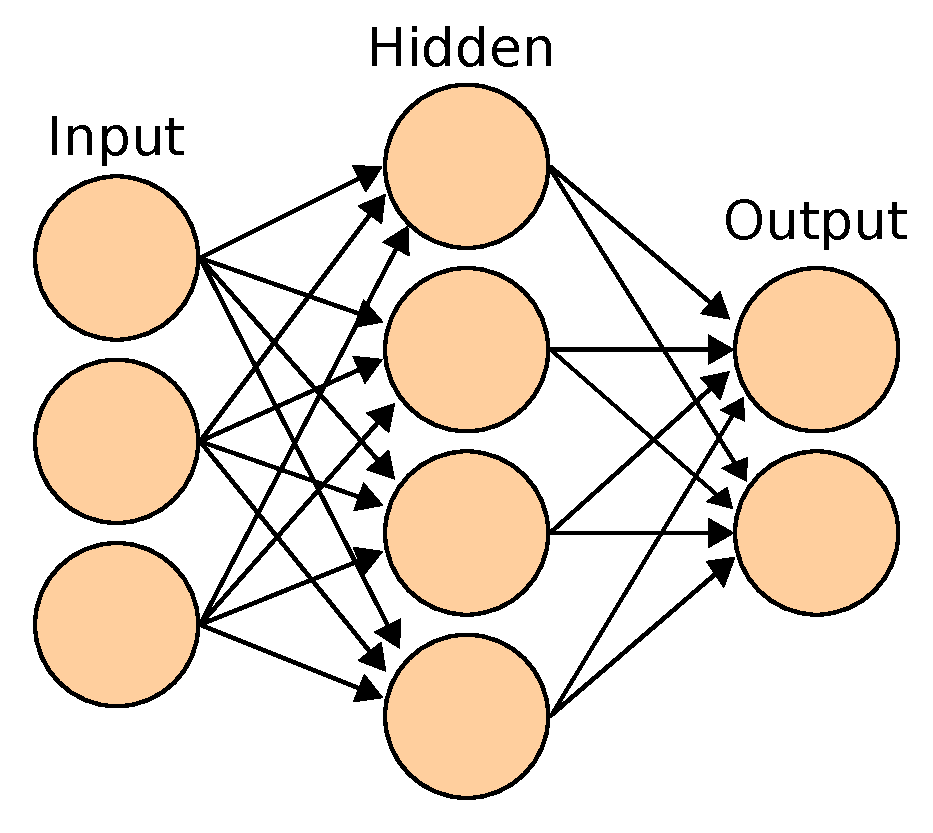
\includegraphics[width=0.5\textwidth]{figures/chapter2/ANN_diagram}
  \caption[Diagram of a typical ANN.]{Diagram of a typical ANN [\cite{ann-wiki-pic}].}
\label{fig:chap2-ann-layout}
\end{figure}

Each network has two special layers, called the input and output layers. The input layer accepts information from which the ANN's designer wants data extracted. The output layer is responsible for producing the output, which contains the information on how the network responded to the input excitation data. In-between these extreme layers lie the so-called `hidden' layers. These layers form the majority of the network and is responsible for interpreting the input data and calculating and producing the networks output. 

The connections between the hidden nodes are represented by a weighting factor which are determined during a training process. These weights define how much influence the nodes have over another, i.e.\ if a weight is positive, it excites another node, whereas if its negative, it suppresses it. The input information traverses the hidden layers, activating the node with the next highest connection weighting. The output data is then determined by which of the nodes were traversed in the hidden layers. The connections between the hidden node layers are mostly responsible for the output and different connection schemes provide different performance characteristics. 

Consider a simple example. You wish to create an ANN that can recognise whether a picture contains a man or a dog. You train it with 25 images of different men and dogs, telling the ANN which picture contains which. Then, after it has been trained, you show it a picture containing a young boy, which is totally unfamiliar to the network. Based on the way you trained it, however, the network should recognise enough human and male features in the child to come to the conclusion that it is more likely that the child is male than it is a dog. 

This ability to classify information that technically falls out of the network's training environment is one of the strengths of ANN's. Other advantages, as stated by~\cite{tu1996advantages}, are ANNs' ability to implicitly detect any non-linear relationships between multi-dimensional input and output dimensions. They can also be trained using different training schemes and modern software packages and libraries have also made it fairly easy to develop a model without any formal statistical training. Some drawbacks of ANN's are that they may require an immense amount of computing power if many nodes are initialised, they are prone to overfitting data when a poorly selected number of nodes are used, and the trained models are extremely `black-box' solutions, making it very difficult to identify and characterise the relationships between the nodes. 

Different ANN topologies and layouts, have been developed and proposed. Some of them are briefly discussed here.

\subsubsection{Feed-forward Network}

The oldest, and arguably the simplest, ANN topography is the feed-forward network (FFN), also referred to as multi-layer perceptron if there are multiple node layers in the hidden layer. Its layout is typically very similar to the layout given in Figure~\ref{fig:chap2-ann-layout}, with a single input and output layer, as well as a single or multiple hidden node layers. 

The FFN uses some form of supervised training algorithm, with the backpropagation algorithm commonly used Here the hidden nodes are adjusted until the output the network produces is as close as possible to the target output specified by the designer. This configurations biggest attractions are its simplicity, relatively fast training speed, depending on the number of hidden layers, and its ability to derive non-linear relationships between dimensions. However, FFN's are prone to converging very slowly, and sometimes getting stuck in local minima, as stated by~\cite{svozil1997introduction}. However, improvements to the backpropagation training procedure have reduced this effect.

\subsubsection{Recurrent Neural Network}

The recurrent neural network (RNN) is a family of neural networks. The hidden nodes of an RNN makes provision for feedback between the different hidden layers and the output layer, which creates an internal state for the network. See Figure~\ref{fig:chap2-rnn-diagram} for a diagram of a RNN topography.

\begin{figure}
 \centering
 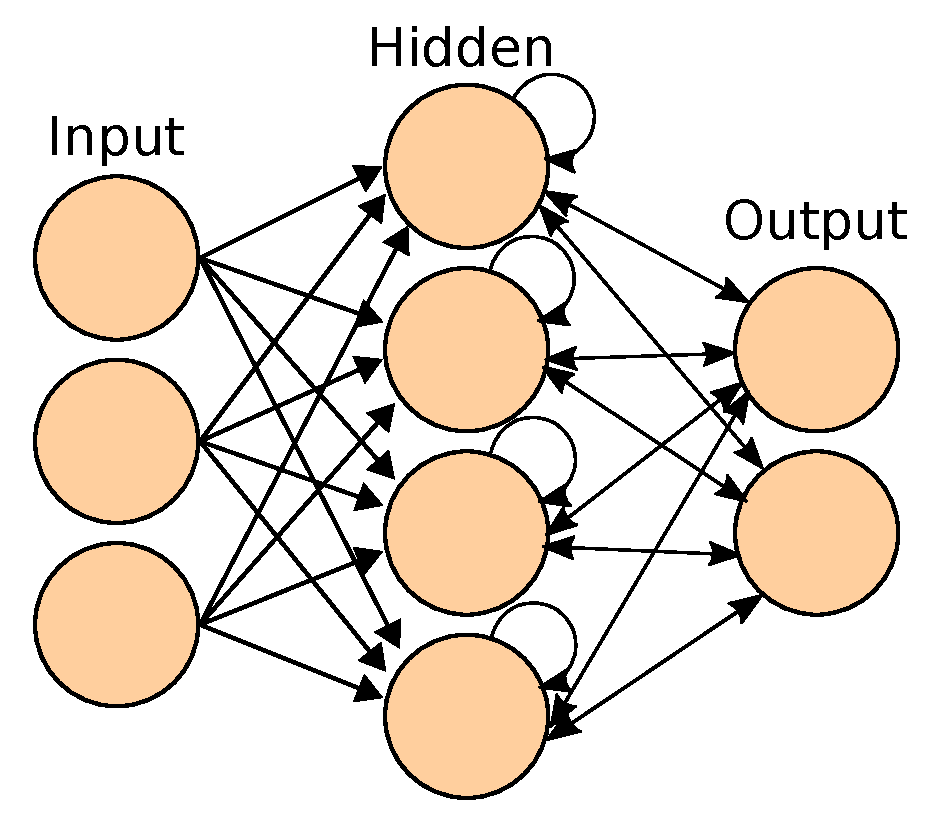
\includegraphics[width=0.5\textwidth]{figures/chapter2/rnn_diagram}
 \caption[A diagram of a simple RNN.]{A diagram of a simple RNN.\@ Adapted from~\cite{ann-wiki-pic}.}
\label{fig:chap2-rnn-diagram}
\end{figure}

In contrast to the FFN, this internal saved state allows the RNN to process arbitrary sequences of input data, making it adept at processing unsegmented speech or handwriting patterns. However, the added complexity of adding feedback loops between the different layers become very expensive computationally, especially when large networks with many layers and inputs are used. Increases in computing power and improvements in the training process, as well as a better general understanding of RNN's and ANN's in general, have alleviated the computational expense somewhat.

There are different RNN configurations available. These include the Hopfield network [\cite{hopfield1982neural}], the echo network [\cite{jaeger2001echo}] and the recurrent multilayer perceptron network [\cite{tutschku1995recurrent}].

\subsubsection{Radial Basis Function Network}

The radial basis function network (RBFN) is a type of neural network and is a sub-family of the RNN family, as stated by~\cite{wilamowski1996implementation}. 

The RBFN topology is fixed to a three-layer architecture, with one input layer, one hidden layer and one output layer. The input layer provides the input. The hidden layer then remaps these inputs to make them linearly separable, where the output layer does the separation and outputs the data [\cite{xie2011comparison}].  

Despite belonging to the same family of ANN, there are a number of significant differences between the RBFN and RNN.\@ Firstly, the three-layer RBFN's are simpler than multi-layered RNN's, making the training process for RBFN's generally faster than that of an RNN.\@ Secondly, and most importantly, as stated by~\citeauthor{xie2011comparison}, is the difference in how the RBFN and RNN classifies the data: the RBFN data clusters are separated by a hyper sphere, whereas the RNN's use arbitrarily shaped hyper surfaces. See Figure~\ref{fig:chap2-classifier} for a demonstration of these class separation strategies. This makes RBFN's an attractive option to interpolate multidimensional data.

\begin{figure*}
  \centering
  \begin{subfigure}{0.5\textwidth}
    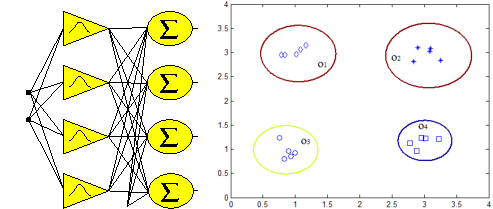
\includegraphics[width=\textwidth]{figures/chapter2/rbf_class}
    \caption{}
    \label{fig:chap2-rbf-classifier}
  \end{subfigure}
  \begin{subfigure}{0.5\textwidth}
    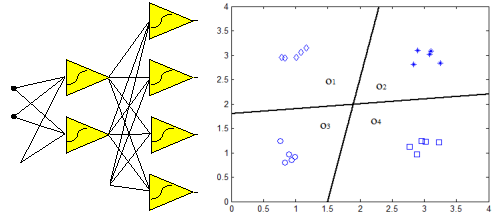
\includegraphics[width=\textwidth]{figures/chapter2/rnn_class}
    \caption{}
    \label{fig:chap2-rnn-classifier}
  \end{subfigure}
  \caption[A comparison between the RBF and RNN classifiers. ]{A comparison between the RBF classifier in Figure~\ref{fig:chap2-rbf-classifier} and the RNN classifier in Figure~\ref{fig:chap2-rnn-classifier} as shown by~\cite{xie2011comparison}. }
\label{fig:chap2-classifier}
\end{figure*}

~\citeauthor{xie2011comparison} went further to determine that RBFN's are ideally suited to interpolate noisy data where the data surfaces contains regular valleys and peaks. In contrast, normal ANN's and RNN's are more effecient for classification problems and for well-conditioned, regularly spaced data. 

As described by~\cite{skala2012radial}, the function on each node is given by Equation~\ref{eq:chap2-rbf}.

\begin{equation}
  \label{eq:chap2-rbf}
  f(\bm{x_j}) = \sum\limits_{j = 1}^{N}\lambda_j \phi(|| \bm{x}_i - \bm{x}_j ||)
\end{equation}

In Equation~\ref{eq:chap2-rbf}, $\lambda_j$ is the node weighting factor which is determined during the model training phase. The function $\phi$ is the radial function which takes the euclidian norm of the distance between the node centre and the input vector as an input. This radial function is variable and the designer can select the function which best describes the data, though a Gaussian radial function, i.e.\ $\phi(r) = e^{-(\frac{r}{\epsilon})^2}$, $r = || \bm{x_i} - \bm{x_j} ||$, is commonly used.  

\subsection{Support Vector Machines}

Support vector machines (SVM) is a widely used classification technique first proposed by~\cite{vapnik1995support}. It works by finding a hyperplane between two data classes that separates the classes by the widest possible average margin. See Figure~\ref{fig:chap2-svm-linear} for an illustration of this separation.

\begin{figure}
  \centering
  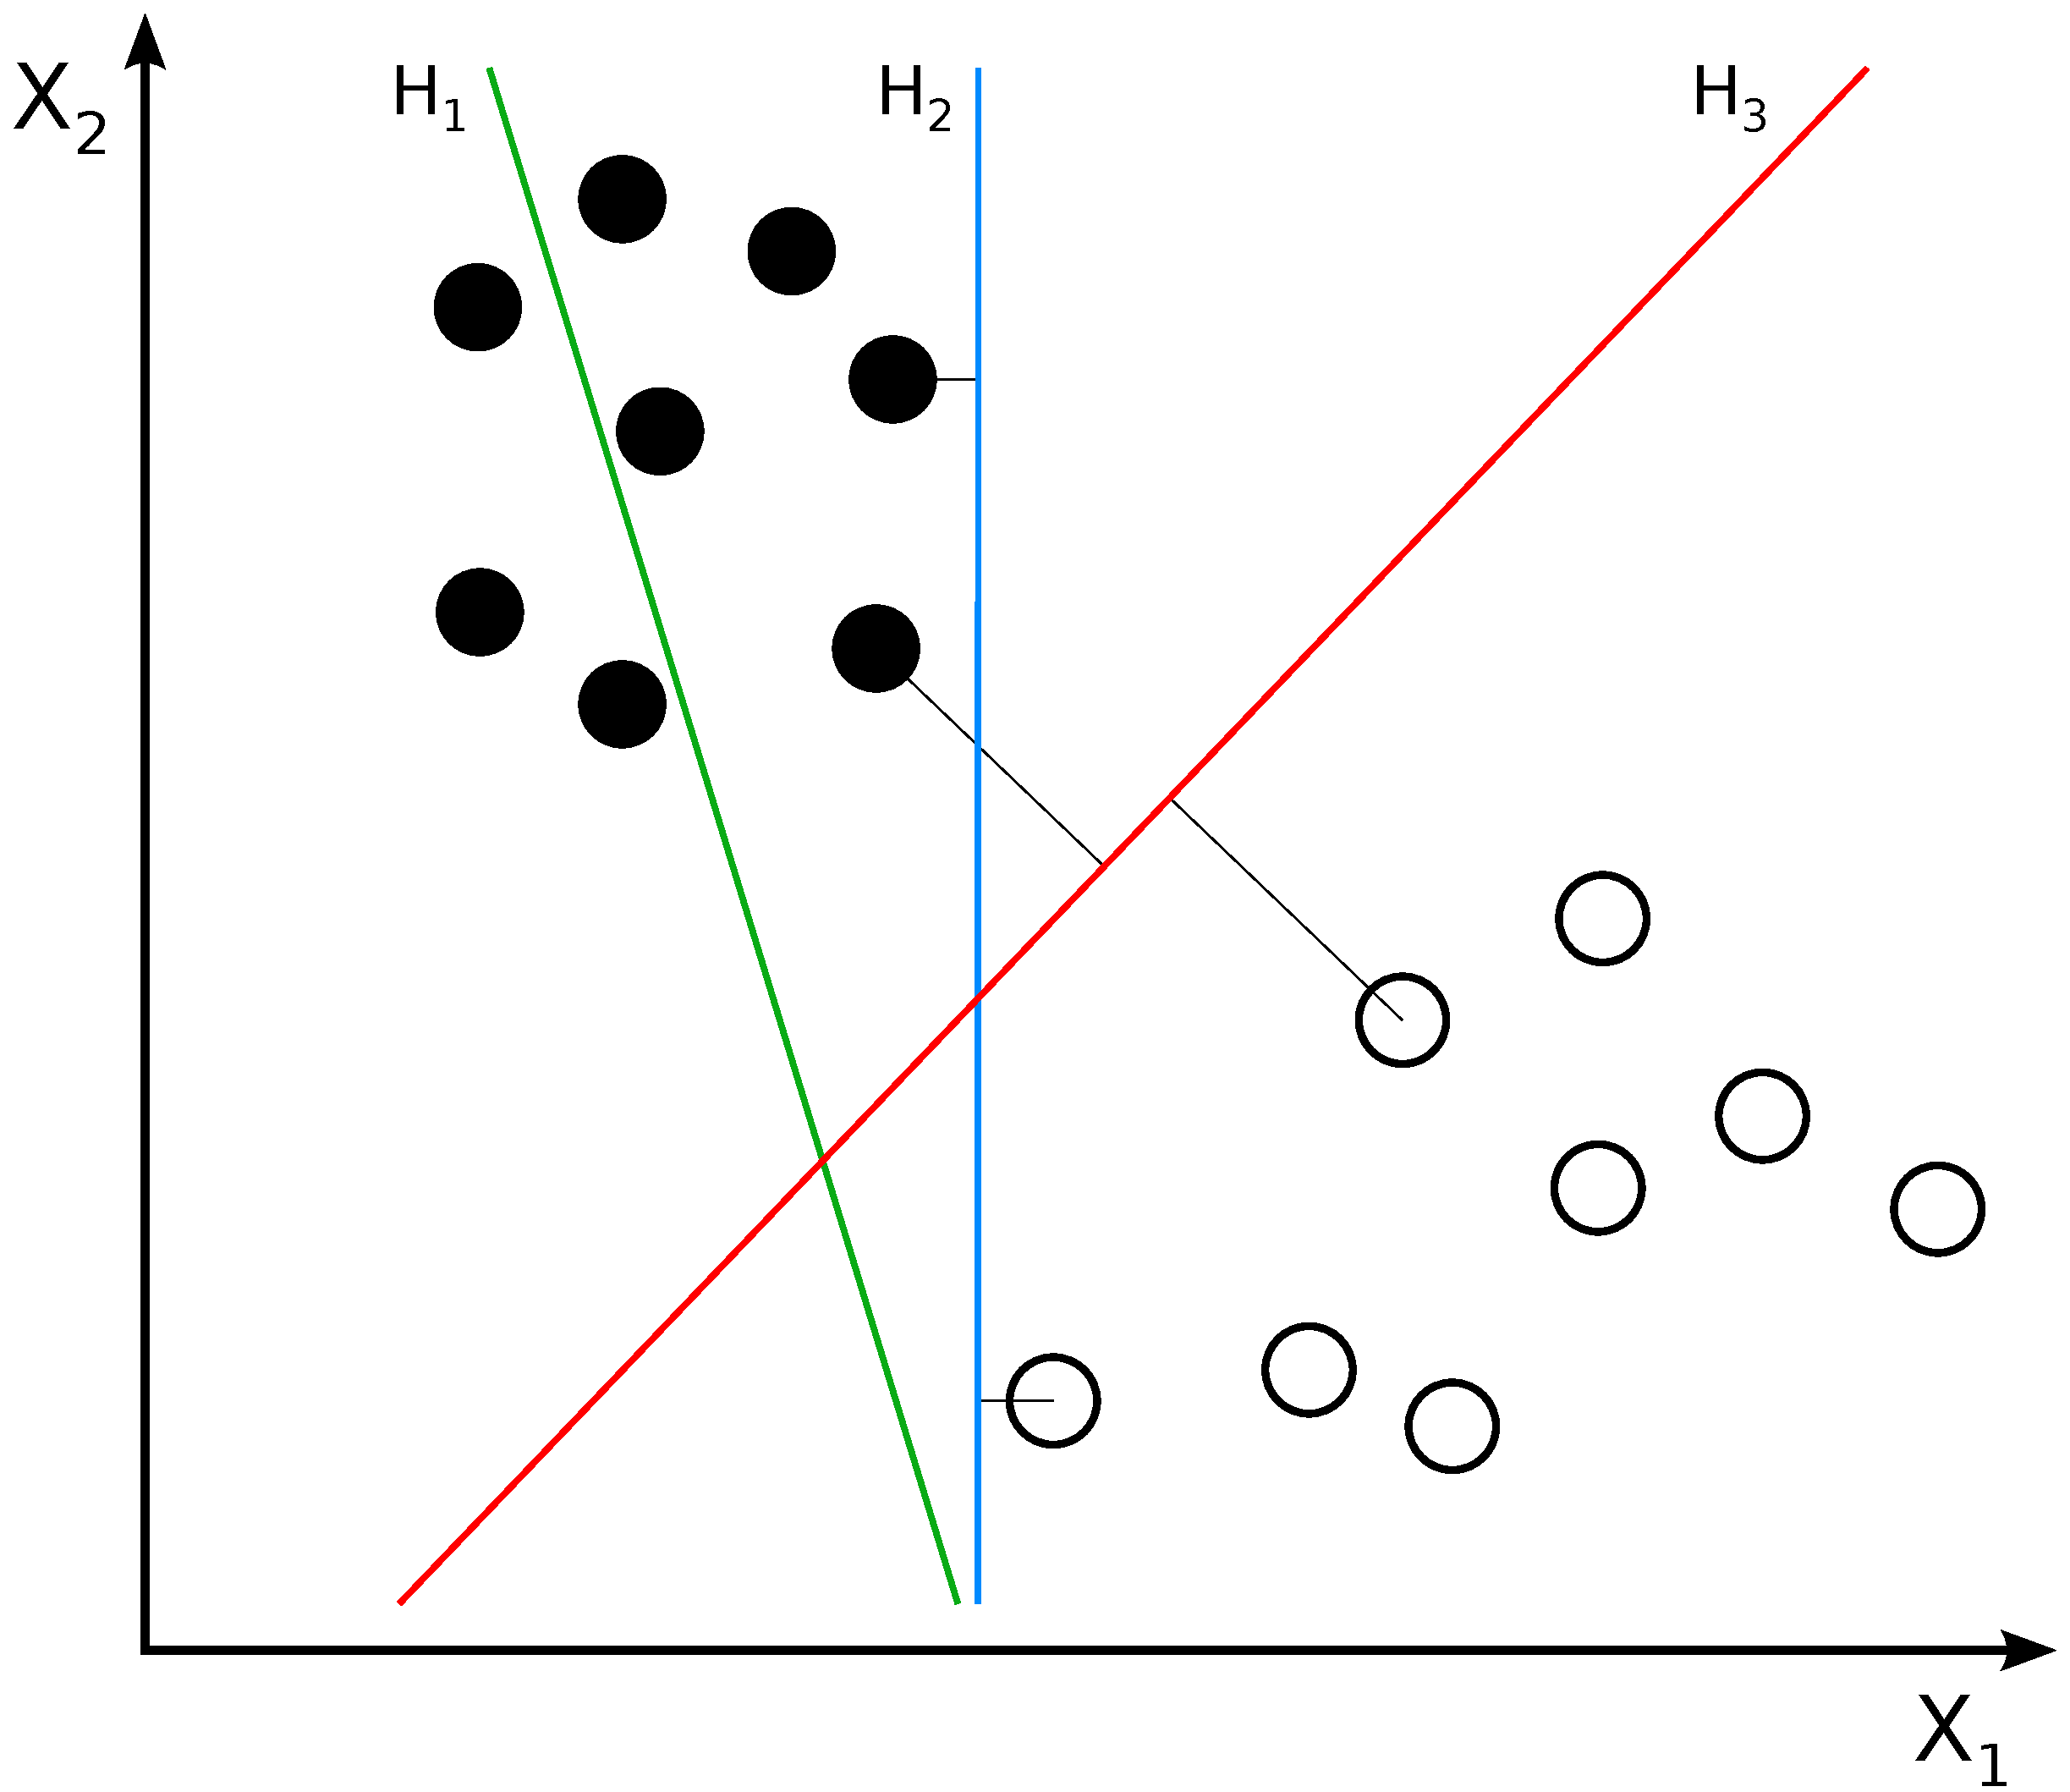
\includegraphics[width=0.5\textwidth]{figures/chapter2/svm_linear}
  \caption[SVM with linear hyperplane.]{SVM plot illustrating different class separators [\cite{svm-wiki-pic}].\@$H_1$ does not separate the classes, while $H_2$ has only minimal class separation. $H_3$ exhibits the widest separation margin.}
\label{fig:chap2-svm-linear}
\end{figure}

\citeauthor{vapnik1995support}'s original method was limited to linear hyperplanes. Since then, the algorithm has extended to be non-linear hyperplanes by applying what is known as the `kernel trick', as described by~\cite{amari1999improving}. An example of such a non-linear separator can be seen in Figure~\ref{fig:chap2-svm-nonlinear}.

\begin{figure}
  \centering
  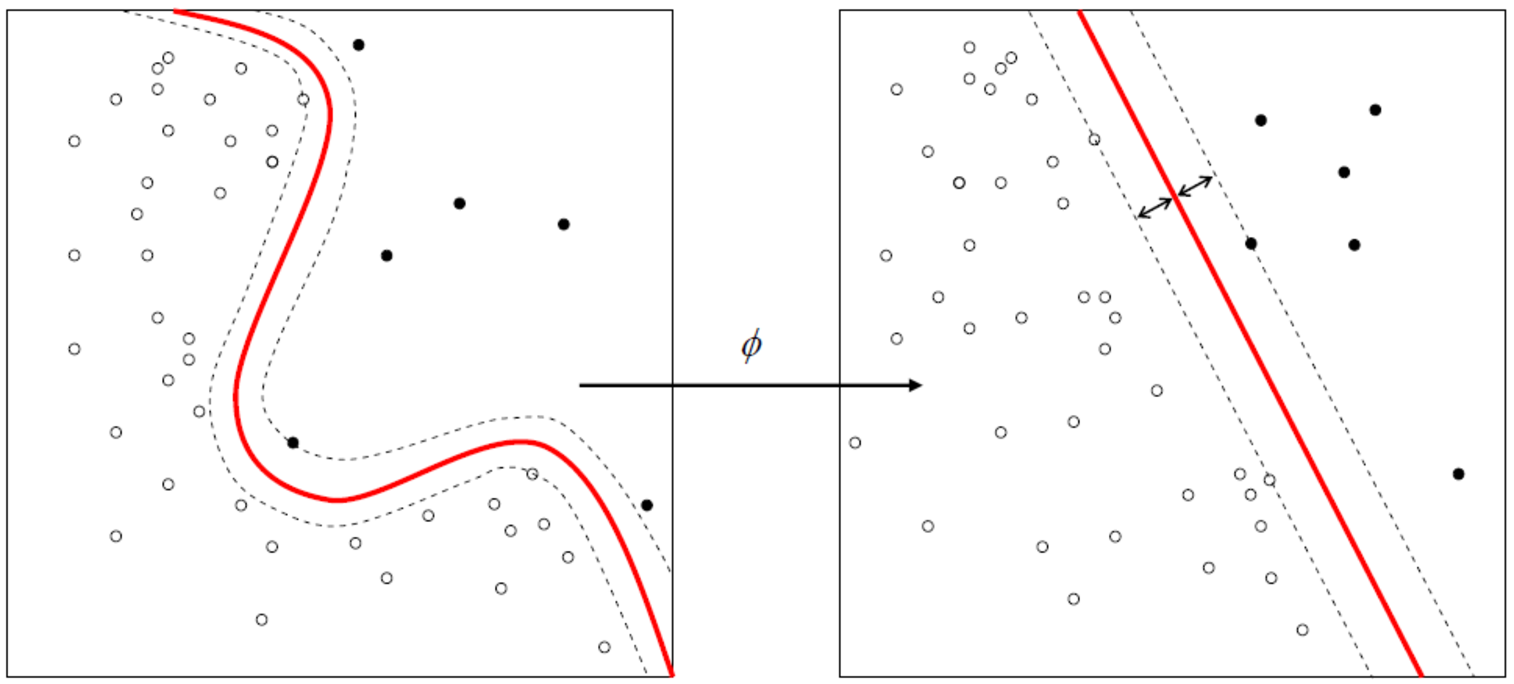
\includegraphics[width=0.8\textwidth]{figures/chapter2/svm_nonlinear}
  \caption[An example of an SVM with a non-linear kernel separator.]{An example of an SVM with a non-linear kernel separator [\cite{kernel-wiki-pic}].}
\label{fig:chap2-svm-nonlinear}
\end{figure}

SVM's are also limited to  binary, i.e.\ two class, problems, somewhat limiting their use for high-dimensional problems. However, they are extremely popular in scientific circles regardless,  thanks to their accuracy and relative simplicity. 
